\section{Enhancement}
\subsection{Unfreezing the word embedding}

As the models we used above are based on the froze pre-trained word embedding which is trained with general corpus, this word embedding may not perform the best on our current corpus. In this section, we will unfreeze the word embedding so that it can better match our current corpus.

\begin{table}[h]
\centering
\caption{Result of the Unfreezing Word Embedding}
\label{tab:unfreeze}
\begin{tabular}{l|llll}
\toprule
                & Test/Acc      & Test/Loss     & Val/Acc       & Val/Loss      \\
\midrule
Unfreeze &  77.01 & 53.29 & 78.42 & 51.82
\end{tabular}
\end{table}

\subsection{Mitigating the OOV word influence}

\begin{table}[h]
\centering
\caption{Result of the OOV strategy}
\label{tab:oov}
\begin{tabular}{l|llll}
\toprule
                & Test/Acc      & Test/Loss     & Val/Acc       & Val/Loss      \\
\midrule
Simple Ignore   & 0.71          & 0.61          & \textbf{0.74} & \textbf{0.60} \\
Greedy Matching & \textbf{0.73} & \textbf{0.60} & 0.73          & 0.61         
\end{tabular}
\end{table}

Our approach to mitigating the out-of-vocabulary (OOV) issue is evaluated using two strategies: simple ignore (replacing OOV tokens with a padding token) and a hash-based greedy matching method, implemented in our code as described in~\cref{alg:HashBasedGreedyMatching}. Both strategies were evaluated on accuracy and loss for the validation and test sets under the same experimental conditions, with the word embeddings unfrozen and trained for 3 epochs.

As shown in Table~\ref{tab:oov}, the greedy matching strategy slightly outperforms the simple ignore method on test accuracy (0.73 vs. 0.71) and test loss (0.60 vs. 0.61). However, the simple ignore method achieves marginally better results on the validation set, with a validation accuracy of 0.74 and validation loss of 0.60. These results suggest that while the greedy matching method is generally more effective on the test set. Though simple ignore performs better on the validation set, it is shows trend to overfit on the test set and may perform even worse on more complex dataset.


\subsection{biLSTM and biGRU}

\begin{table}[h]
\centering
\caption{Result of the biLSTM and biGRU}
\label{tab:bilstm}
\begin{tabular}{l|llll}
\toprule
                & Test/Acc      & Test/Loss     & Val/Acc       & Val/Loss      \\
\midrule
biLSTM & 0.77 & 0.53 & 0.79 & 0.52\\
biGRU & 0.78 & 0.53 & 0.78 & 0.52
\end{tabular}
\end{table}

Table~\ref{tab:bilstm} presents the performance results for the biLSTM and biGRU models. The biLSTM achieves a test accuracy of 0.77 with a test loss of 0.53, while its validation accuracy and loss are 0.79 and 0.52, respectively. The biGRU model shows slightly higher test accuracy at 0.78 with the same test loss of 0.53, and its validation accuracy and loss are 0.78 and 0.52, respectively.

\subsection{CNN}

Our CNN model achieves a test accuracy of 0.77 and a test loss of 0.54, with a validation accuracy of 0.77 and validation loss of 0.52, as shown in Table~\ref{tab:cnn}. The hyperparameters were optimized using a WandB agent to ensure the model’s best performance under our experimental conditions.

\begin{table}[h]
\centering
\caption{Result of the CNN}
\label{tab:cnn}
\begin{tabular}{l|llll}
\toprule
                & Test/Acc      & Test/Loss     & Val/Acc       & Val/Loss      \\
\midrule
CNN & 0.77 & 0.54 & 0.77 & 0.52
\end{tabular}
\end{table}

\subsection{Model enhancement}

\begin{table}[bt]
\centering
\caption{The result of our enhancement method}
\label{tab:enhance}
\begin{tabular}{l|llll}
\toprule
         & Test/Acc      & Test/Loss     & Val/Acc       & Val/Loss      \\
\midrule
Baseline & 0.72          & 0.59          & 0.75          & 0.58          \\
w. Attn  & \textbf{0.74} & \textbf{0.57} & \textbf{0.76} & \textbf{0.55}
\end{tabular}
\end{table}

We incorporate a self-attention mechanism prior to the aggregation step to leverage global information from each token, aiming to enhance the model's ability to capture contextual dependencies. The impact of this approach is shown in Table~\ref{tab:enhance}, where we compare the baseline model with and without self-attention.

The model with self-attention (denoted as ‘w. Attn’) outperforms the baseline across both validation and test sets. Specifically, it achieves a test accuracy of 0.74 and a test loss of 0.57, compared to 0.72 and 0.59 for the baseline. On the validation set, the self-attention model yields an accuracy of 0.76 and a loss of 0.55, surpassing the baseline's accuracy of 0.75 and loss of 0.58. These results suggest that integrating self-attention enhances the model's performance by effectively capturing token-level interactions, which improves generalization on unseen data.

\subsection{Discussion}

\begin{figure}
    \centering
    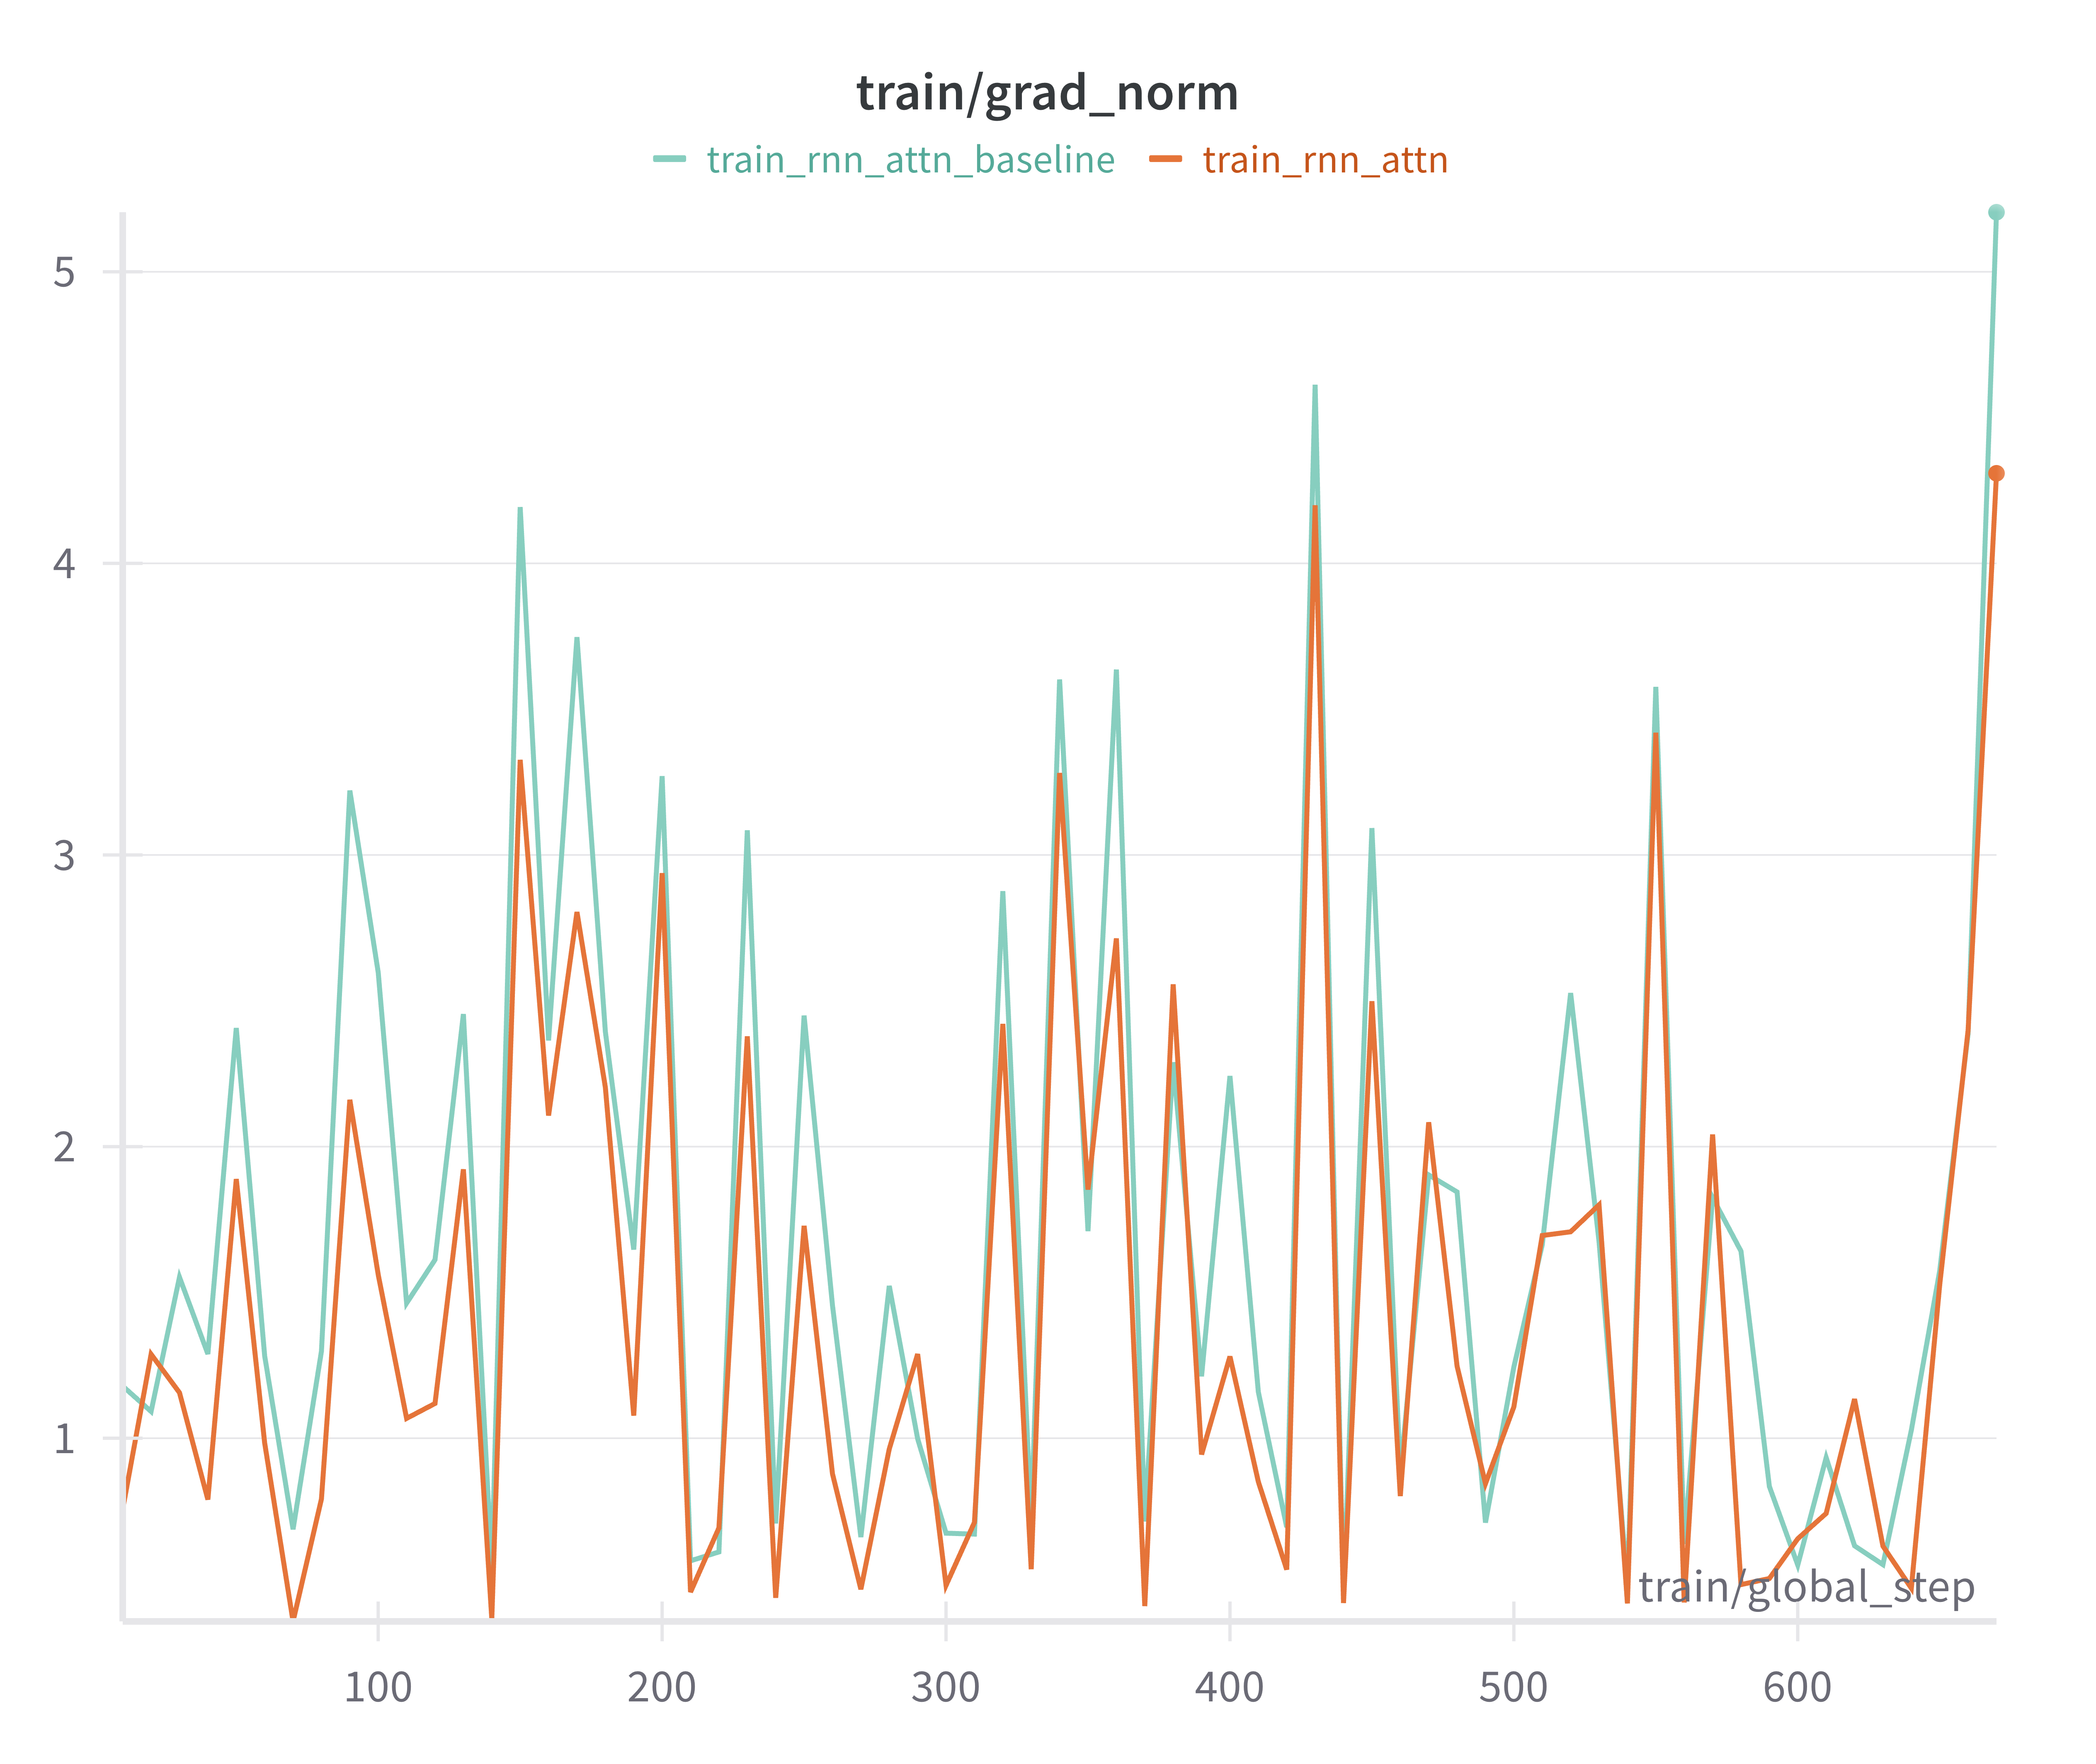
\includegraphics[width=0.75\linewidth]{images/grad_norm.png}
    \caption{A demonstration of the gradient norm in our training process}
    \label{fig:grad-norm}
\end{figure}

In this subsection, we summarize our findings from previous experiments and discuss factors that may have influenced the model's performance.

\paragraph{Vocabulary Size} We believe vocabulary size significantly impacts model performance. In our ablation studies, using a smaller GloVe embedding yielded worse results compared to a larger version under the same settings. With only around 1\% of tokens in the test set facing out-of-vocabulary (OOV) issues, the model can still extract substantial information from the pretrained GloVe vocabulary. Consequently, our strategy for addressing OOV issues provided only minimal improvements.

\paragraph{Dataset Size} The dataset contains approximately 8,000 rows, which limits the distribution from which the model can learn. Even if the model is scaled, without leveraging domain-specific knowledge from large pretrained models such as BERT, training from scratch remains challenging on such a small dataset.

\paragraph{Parameter Tuning} Parameter tuning proved to be particularly impactful with this small dataset. We suspect that due to the limited data distribution, the loss landscape is sharp, making convergence to a stable minimum challenging. An example of the gradient norm using the RNN is shown in~\cref{fig:grad-norm}. As illustrated, the gradient norm fluctuates significantly, indicating large steps taken by the optimizer and highlighting the difficulty of achieving stability